\begin{frame}[allowframebreaks]{Convolution-Summe}

    %---------------------------------------------
    % Herleitung ueber Summe verz. Einheitsimpulse 
    %---------------------------------------------
    Jedes diskrete Signal kann als Summe skalierter, verzögerter Einheitsimpulse dargestellt werden \cite{oppenheim1999}.

    \begin{figure}
        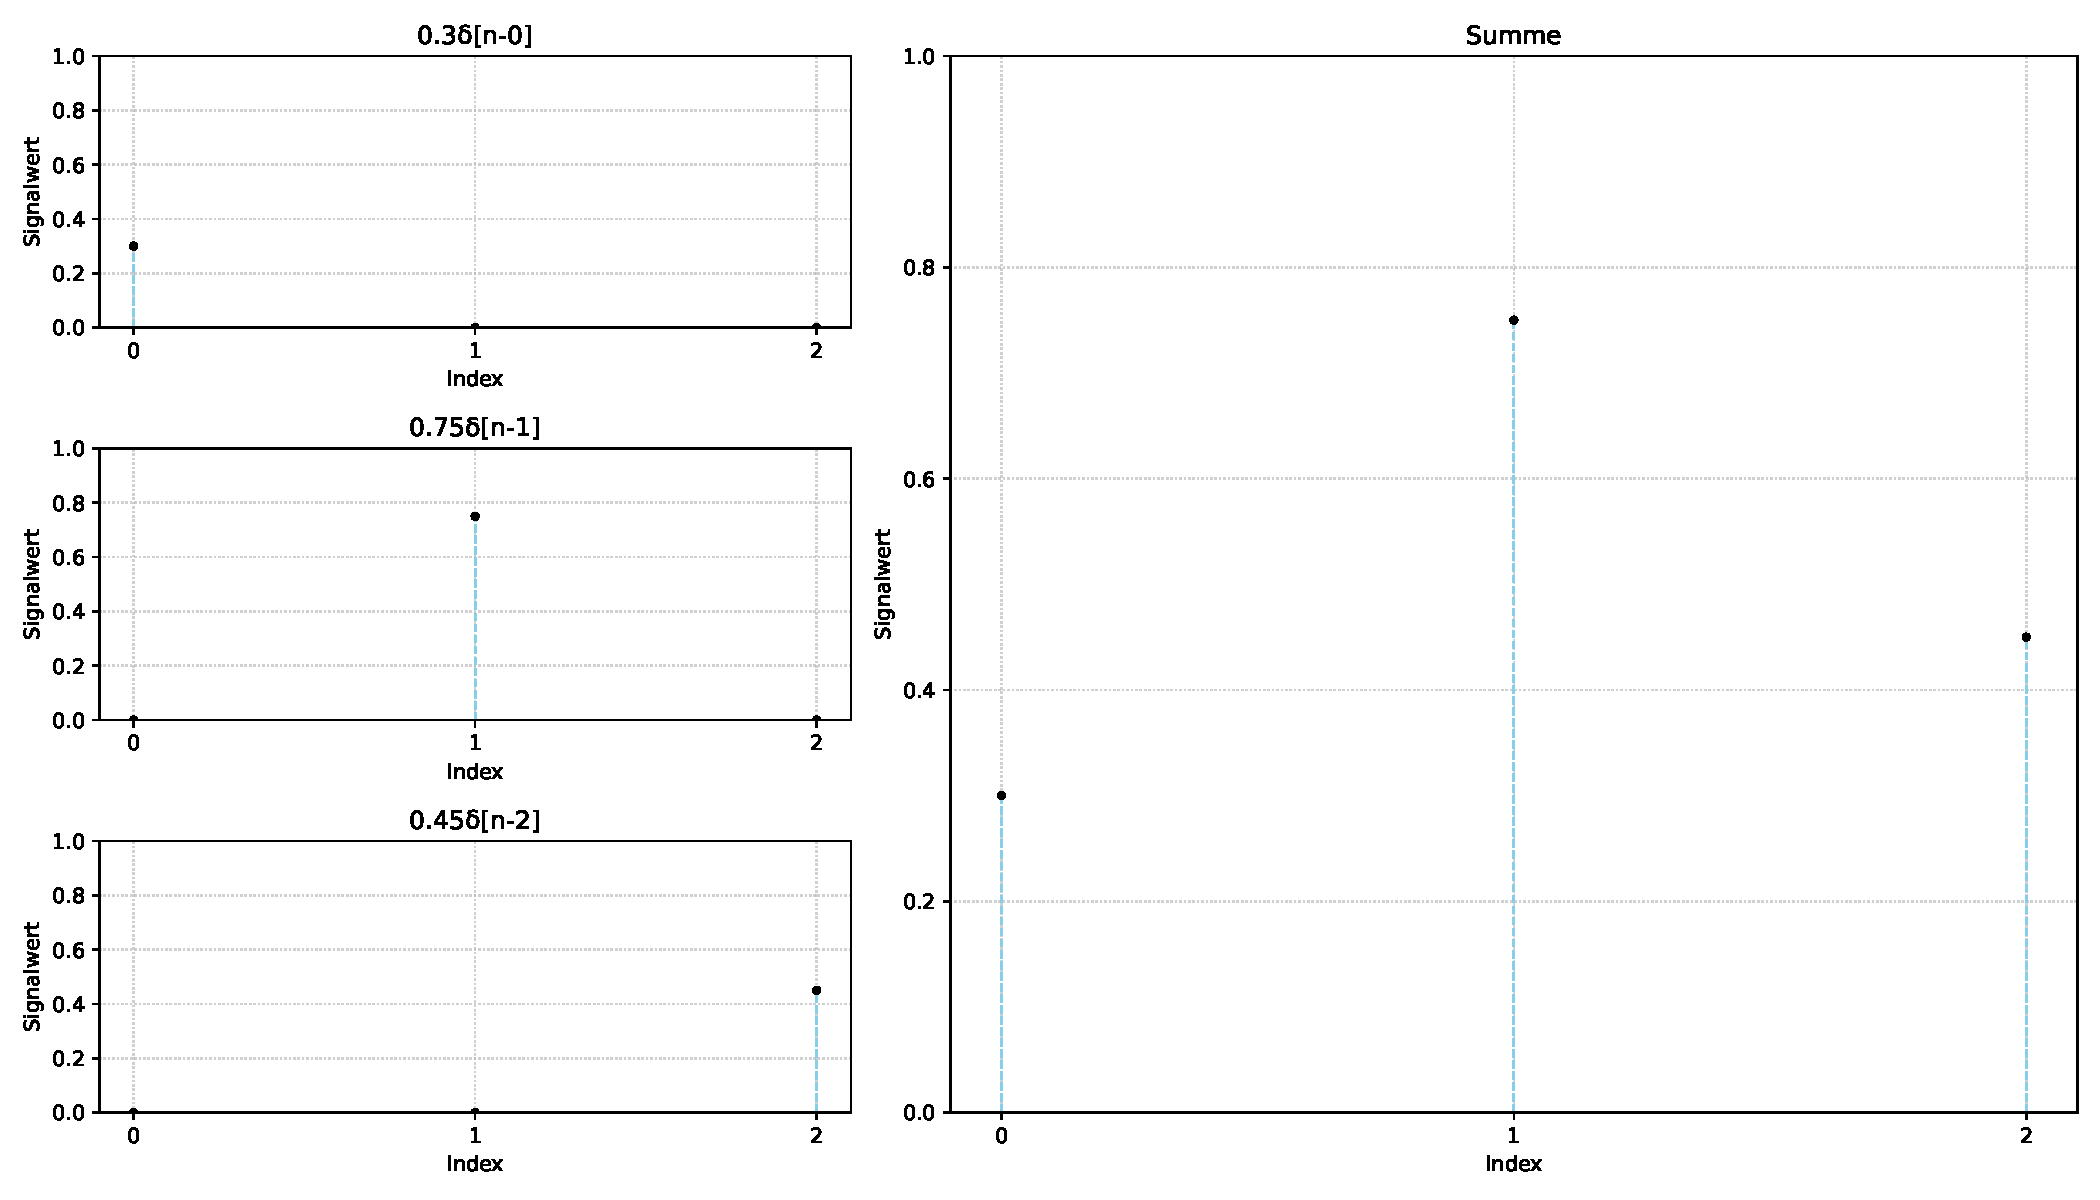
\includegraphics[width=0.75\textwidth]{Graphics/signals_sum.pdf}
        \centering
        \caption{Summe dreier skalierter, verzögerter Einheitsimpulse}
    \end{figure}

    \framebreak

    Diskretes Signal als Summe skalierter, verzögerter Einheitsimpulse:

    \begin{equation}
        x[n]=\sum_{k=-\infty}^\infty x[k]\delta[n-k]
        \label{eq:scaled_unit_sum}
    \end{equation}

    \framebreak

    Anwenden einer Transferfunktion $T$ auf ein Signal:

    \begin{equation}
        y[n]=T(x[n])=T\left(\sum_{k=-\infty}^\infty x[k]\delta[n-k]\right)
    \end{equation}

    \framebreak

    Für lineares System gilt:

    \begin{equation}
        y[n]=\sum_{k=-\infty}^{\infty}x[k]T(\delta[n-k])=\sum_{k=-\infty}^{\infty}x[k]h_k[n]
    \end{equation}

    \begin{itemize}
        \item $h_k$: Transferfunktion eines Systems bei Eingangssignal $\delta[k]$ an Index $n$
        \item System könnte unterschiedlich auf Einheitsimpulse an verschiedenen Indizes reagieren
    \end{itemize}

    \framebreak

    Für Lineares Zeit-Invariantes System gilt:

    \begin{equation}
        y[n]=\sum_{k=-\infty}^{\infty}x[k]h[n-k]
    \end{equation}
    \begin{itemize}
        \item Convolution-Summe
        \item Wann $h[n]$ bestimmt wurde ist nicht mehr relevant!
        \item Kurzschreibweise: $y[n]=x[n]*h[n]$
    \end{itemize}

\end{frame}

\begin{frame}[allowframebreaks]{Moving Average Filter}

    Anschauliches Beispiel für Convolution-Summe: Moving Average Filter (Low-Pass FIR-Filter)
    \linebreak
    \begin{itemize}
        \item Werte von $y[n]$ berechnet aus Mittelwert einiger Werte aus $x[n]$
    \end{itemize}
    
\framebreak

\begin{figure}[H]
    \centering
    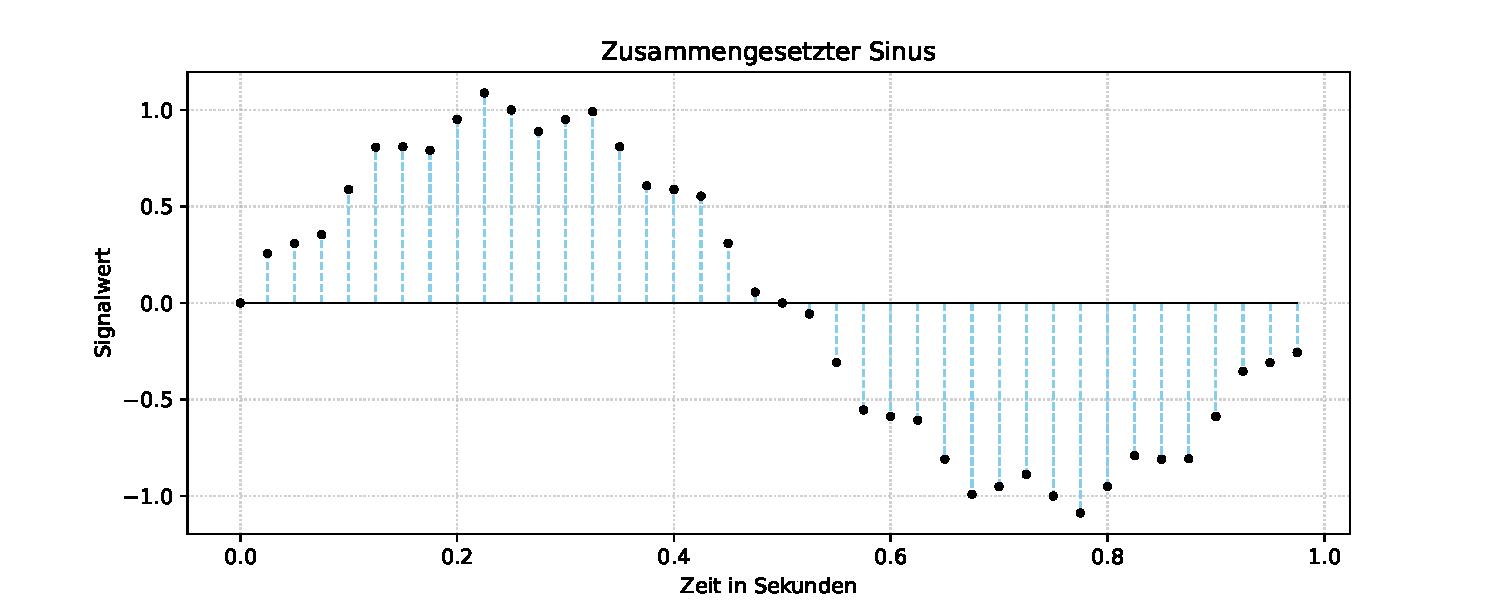
\includegraphics[width=0.8\textwidth]{Graphics/compound_sinusoid.pdf}
    \caption{Ein diskretes Signal, zusammengesetzt aus Sinusschwingungen mit den Frequenzen $f_0=1\,\text{Hz}$, $f_1=10\,\text{Hz}$, und $f_2=20\,\text{Hz}$}
    \label{fig:comp_sinusoid}
\end{figure}

\framebreak

\begin{figure}[H]
    \centering
    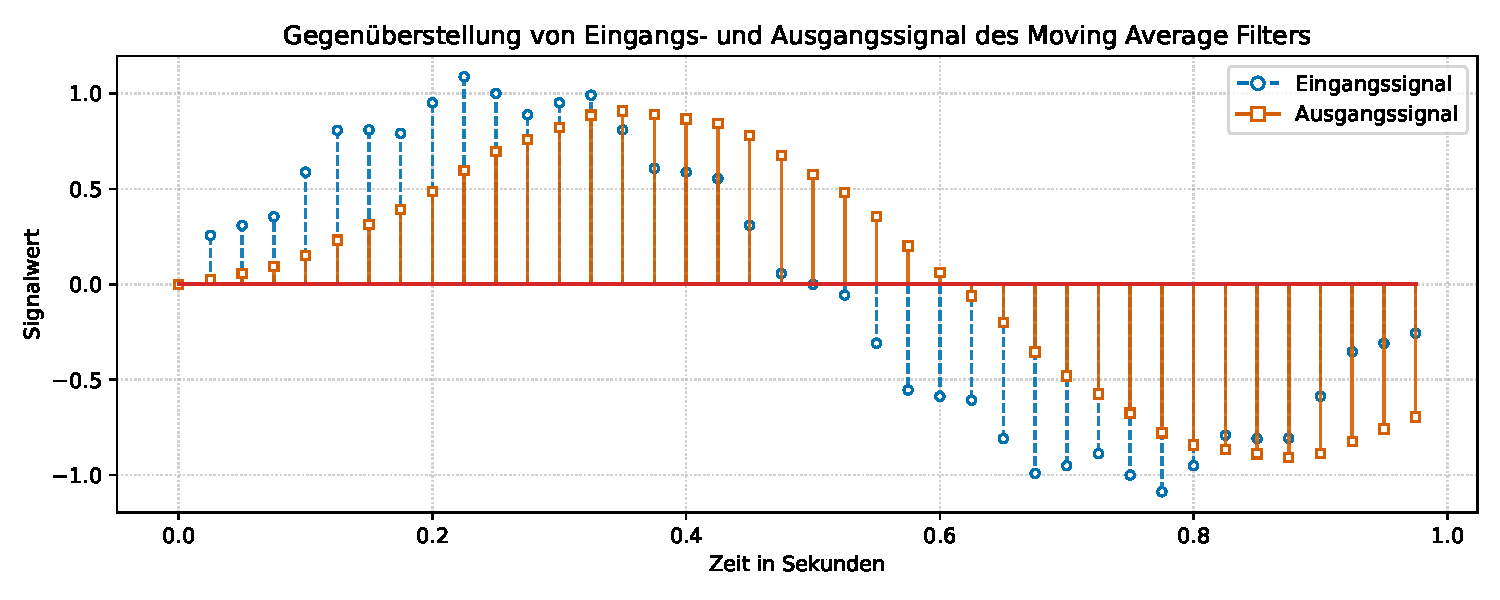
\includegraphics[width=0.8\textwidth]{Graphics/comparison_compound_filtered.pdf}
    \caption{Dasselbe diskrete Signal, Ausgangssignal des Moving Average Filters überblendet}
    \label{fig:filtered_sinusoid}
\end{figure}

\framebreak

Es werden $m$ Samples summiert, und das Ergebnis mit $\frac{1}{m}$ multipliziert:

\begin{equation}
    y[n]=\frac{1}{m}\sum_{k=0}^{m-1}x[n-k]\iff y[n]=\sum_{k=0}^{m-1}\frac{1}{m}x[n-k].
    \label{eq:mov_avg_filter}
\end{equation}
\cite[S. 172]{lyons2011}.

\framebreak

Koeffizienten $\frac{1}{m}$ können als Folge der Länge $m$ mit dem Wert $\frac{1}{m}$ an jedem Index interpretiert werden. Zum Beispiel für $m=5$:

\begin{equation}
    \label{eq:fir_convsum}
    y[n]=\sum_{k=0}^4h[k]x[n-k]\text{ mit }h=\left(\frac{1}{5},\,\frac{1}{5},\,\frac{1}{5},\,\frac{1}{5},\,\frac{1}{5}\right).
\end{equation}
\linebreak
$h[n]$ ist die Impulsantwort des FIR-Filters!
\cite[S. 172f]{lyons2011}

\framebreak

Die Impulsantwort ist das Ausgangssignal des Systems (hier Moving Average Filter) bei einem Eingangssignal $\delta[n]$.

\end{frame}

    %---------------------------------------------
    % Convolution-Theorem
    %---------------------------------------------

\begin{frame}[allowframebreaks]{Convolution-Theorem}

    Für Signale $x[n], y[n], h[n]$ seien $X(e^{i\omega})$, $H(e^{i\omega})$ und $Y(e^{i\omega})$ die Repräsentationen der Signale in Frequenzdomäne.  

    Es gilt:
    \begin{equation}
        Y(e^{i\omega})=X(e^{i\omega})\cdot H(e^{i\omega}).
    \end{equation}

    \begin{itemize}
        \item Die Berechnung der Convolution-Summe zweier Signale in Zeitdomäne ist äquivalent zum Produkt der Signale in Frequenzdomäne.
    \end{itemize}
        
\end{frame}